\chapter{Background}
    In this chapter, we introduce the context of the work to give the reader an understanding of its importance, and then the concepts used during the experiments both withing acoustics and machine learning.
    
    
\section{Marine advisory work}
    The \gls{ices} is an intergovernmental science organization that is the primary provider of advice on marine ecosystems to the governments and international bodies that manage the North Atlantic Ocean and adjacent seas\cite{ICES2020}. It consists of over 6000 marine scientists, over 300 institutes and 20 member countries, where Norway is one of them. Advice is developed by expert groups who work towards better understanding of marine ecosystems and their sustainable use. The \gls{imr} is a large contributor, and one of its activities is to give input to these advices through research and monitoring. An important research area is the monitoring of a species known as the \textit{lesser sandeel}, which is the area in which this thesis seeks to contribute.
    
\subsection{Why the lesser sandeel?}
    The lesser sandeel (\textit{Ammodytes marinus}), from now just \textit{sandeel} is
    a small pelagic \footnote{Pelagic fish inhabit in the pelagic zone of ocean or lake waters – living neither close to the bottom nor near the shore.} fish which resides in sandy-bottomed coastal and shallow ocean waters and feeds mainly on plankton. It plays a key role in the North Sea, as it has a major role in the marine ecosystem as forage fish\footnote{Forage fish are small pelagic fish which are preyed on by larger predators.} and catch for fisheries. Due to the high level of predation, it lives large parts of its life buried in a sandy seabed, but during the spring feeding season adults emerge each dawn to create large schools in the upper pelagic layer. Historic data show that changes in their abundance cause bottom-up effects of the ecosystem, causing for example breeding failure among several species of seabird \cite{johnsen2017collective}. 
    
    The North Sea is under pressures, stemming from a range of factors including fishing, coastal construction, maritime transport, oil and gas exploration and production, tourism and recreation, navigation dredging, aggregate\footnote{Raw materials such as gravel, crushed stone, or sand that are obtained from natural sources.} extraction, military activities, and wind farm construction \cite{ICES2021}. Because of the importance of sandeel, \gls{imr} has conducted yearly acoustic trawl missions since 2005 in sandeel areas of the North Sea\cite{johnsen2017collective}. The goal is to monitor the sandeel stock and create input and data to help the \gls{ices} create scientifically backed advice, one of which are recommendations for fishing quotas\cite{sizedependentfreqrespons2009johnsen}. 
    
    \begin{figure}[H]
        \centering

        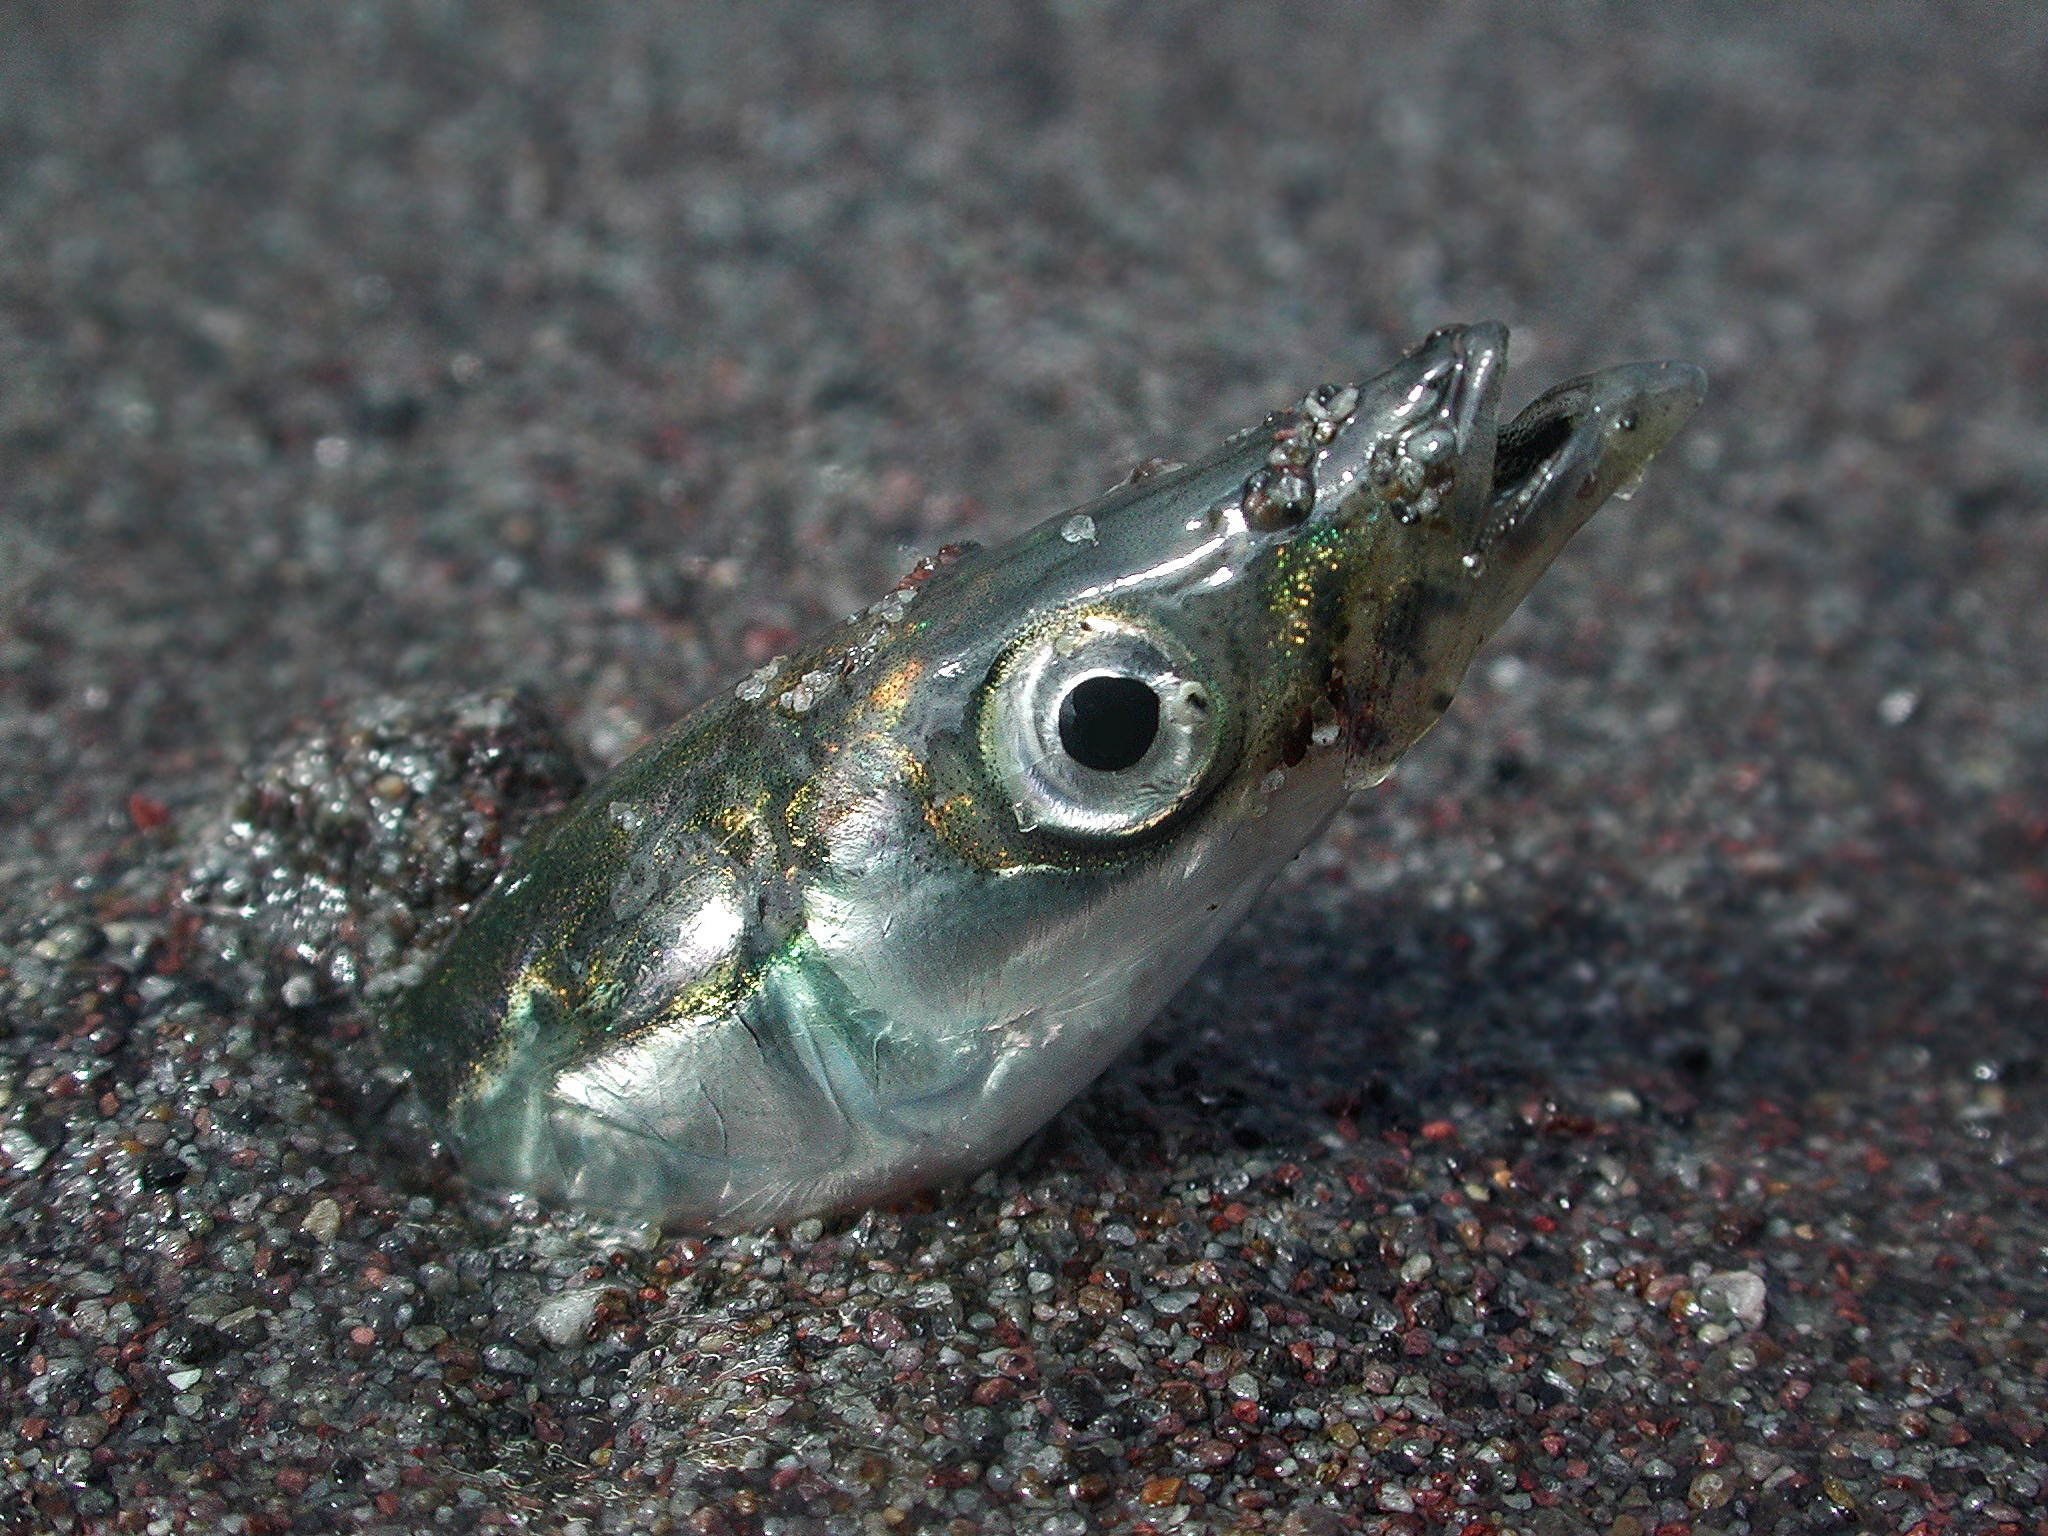
\includegraphics[width=0.5\textwidth]{figures/Ammodytes_hexapterus.jpg} 

        \caption[Sandeel]{A sandeel buried in sand.}
        \medskip 
        \hspace*{15pt}\hbox{\scriptsize Credit: Original image by Mandy Lindeberg\cite{sandeel_image}}
        \label{sandeel_image}
    \end{figure}



    
\section{Acoustics surveys}\label{acoustics}
    When fisheries conduct acoustic surveys of fish, they use \textit{echo sounders} to remotely detect and observe targets in the water. Echo sounders are a special variety of \textit{sonar}, where the acoustic beam is directed vertically downwards from the measuring platform. The echo sounder consists of a \textit{transmitter} that produces a burst of electrical energy at some set frequency. Then a \textit{transducer} receives the output from the transmitter and converts it to an acoustic signal that is propagated through the water, this signal is also called a \textit{ping}. This forms a directional beam, akin to the light from a handheld flashlight. Targets in the water \textit{backscatters}/\textit{reflects} parts of the energy back towards the transducer. The backscattered sound or \textit{echo} is detected by the transducer, and the sound is converted back to electric energy as the received signal and is further amplified. The time when the signal is received determines the range to the target\cite{simmonds2008fisheries}.
    
    Pings are usually represented as columns in a 2-dimensional image, also called an \textit{echogram}, with range along the y-axis and time of ping along the x-axis. The columns represent how the acoustic reflections varies for each ping. Any targets detected in the ping will be visualized as a mark in the echogram, usually with different colors depending on the echo strength. In multi-frequency sonars, individual echograms are produced in parallel for each frequency in use, this is visualized in figure \ref{echogram_example_fig}. Because the echograms are constructed as $\text{time} \times \text{range}$, the vertical magnitude of a mark indicates the height of the target, while the horizontal position illustrate changes in \textit{time} if the echosounder is stationary or in \textit{space} if moving. When moving, the echogram thus represents a vertical cross-section of the water column as the transducer is in motion through the water at constant speed in one direction\cite{simmonds2008fisheries}.
    
    %If the echosounder was stationary, the echogram would be a time-series representation of the same volume. Combined with trawl samples and knowledge of species composition, the mark can be assigned to a specific or group of species.
    
    \begin{figure}[H]
        \centering
            \includesvg[inkscapelatex=false,width=1\textwidth,keepaspectratio]{figures/echogram-echosounder.svg}
        \caption[Echosounder]{Concept of an echosounder: Pings generates echoes from a school of fish and the seabed. The echoes are displayed in an echogram.}
      	\medskip 
        \label{echogram}
    \end{figure}
    
    \begin{figure}[H]
        \centering
            \includesvg[inkscapelatex=false,width=1\textwidth,keepaspectratio]{figures/acosutic_data.svg}
        \caption[Echosounder]{Example echograms from multiple frequencies.}
      	\medskip 
        \label{echogram_example_fig}
    \end{figure}

%\subsection{Acoustic Propagation and Noise}
    
\subsection{Acoustics and Fish}
    To measure the force of backscattered sound received from a target, the backscattered cross-section or the \gls{ts} are used. They are defined as:
    
    \begin{equation}
        \sigma_{bs} = r^{2}\frac{I_{b}}{I_{i}},
    \end{equation}
    

    \begin{equation}
        \textrm{TS} = 10 \log_{10}(\sigma_{bs}),
    \end{equation}
    where $I_{b}$ is sound intensity backscattered from the target, $I_{i}$ is the intensity of the ping at some arbitrary distance (usually 1m) and \textit{r} is the distance away from the transducer($\sigma_{bs}$ in units $m^{2}$). $\sigma_{bs}$ can vary greatly depending on the frequency used, or the composition, angle and shape of the target and several other factors as described in \citet{simmonds2008fisheries}. 

\subsection{The Volume Backscattering Coefficient}
    Individual targets in some sampled volume may be small and plentiful, resulting in their echoes combining and forming a continuous backscattered signal with varying amplitude. Single targets are no longer possible to distinguish, but the signal itself is a measure of the biomass in the water watercolumn. This is measured using the \gls{sv} defined as:
    
    \begin{equation}
        s_{v} = \sum \sigma_{bs} / V_{0},
    \end{equation}
    
    where a sum over all discrete targets returning echoes in the sampled volume ($V_{0}$) is taken. There is a linear relationship between the abundance of fish, and \gls{sv} as long as the species or group of species is known. For more details, see \citet{simmonds2008fisheries}.

\subsection{IMRs acoustic trawl surveys}
    \gls{imr}s acoustic trawl missions combine the gathering of acoustic data and biological data from trawl catches. The scrutiny of the data is done through the use of a post-processing software called \gls{lsss}, where acoustic target classification is done \textit{manually} with the biological samples as aid\cite{korneliussen2006large}. The echogram for each frequency channel used is stored as a 2-dimensional picture, where each pixel value is a \gls{sv} value.  Afterwards, the data and biological samples are input to a software called StoX.  This is an open-source software which is used to estimate the fish abundance and age distribution to be further used as support for \gls{ices} advice\cite{johnsen2019stox}. \cite{korneliussen2018acoustic}




%    Hei,
%Det finnes en del på dette (se under). Vi bruker 200 kHz når vi finner stimer, men vi %ser at 18KHz og 38 KhZ er viktige for klassifiseringen. 
%
%\citet{sizedependentfreqrespons2009johnsen} - In earlier mentioned annual Norwegian %sandeel surveys the 
%
%\cite{johnsen2017collective} - Bottomconntected schools
%
%\citet{Greenstreet} - 38kHz was adequate but not optimal, with 120kHz as help %discrimination. Sandeels provide a better acoustic return at higher frequencies. 
%
%\citet{pedersen2009relative} - several analyses fish can have species specific reflected %spectrum. backed by. \
%
%\citet{mohammed2006acoustic} - Investegated 18, 38, 120, and 200 kHz. Combinations of sv %can be used to efficiently discriminate between sandeel from herring and mackerel. %Frequency respons instead of relative was better, and more imporant than position and %shape (støtter translation invariance). Some weakness around the use of sv, and better %to use the entire school echo. 
%
%\citet{korneliussen2008proposals} - Multifrequency use can give more information about %acoustic targets. 
%
%\citet{Forland2014Broadbandwidth} - The backscatter from sandeel vary with its %orientation. Causes a behavior where they do not always swim horizontally, slim bodies %,increases the difficulty of interpretating State: Relative low TS because of their lack %of swimmingbladder. backstatter increases with fish size and frequency. Measured the %backscatter of different bodyparts. Many studies have been conducted to find estimates %of sandeel TS at different freqs, but many studies are hard to make use of. %\citet{yasuma2009density} - Back the angle problem, drastic variation in TS by body %length. 
%
%\cite{FREEMAN2004141} - QTC VIEW was used to identify acoustic changes in the properties %of the seabed in the presence of buried sandeels, whilst the EK500 simultaneously %recorded temporal changes in their distribution throughout the water column.
%
%
%OKEIDA SKRIV OM TARGET STRENGTH

%\section{Accoustic Classification of Sandeel (ammodytes marinus)}
%
%https://academic.oup.com/icesjms/article/66/6/1100/694183?login=true 
%- Size-dependent frequency response of sandeel schools
  %  - historically hard to identify because no swim-bladder
  %  - 200kHz for schools, 18 og 38 for individ-classifying
  %  - some work shows:
   %     - some difficulty classify schools og sandeel at 38 and 120kHz
   %     - combinations of Sv at 18, 38, 120, and 200 kHz can effectively identify schools of %sandeel vs. mackerel and herring
   % - goal
   %     - The objective of this study was to identify and exploit differences in frequency %responses to classify sizes of sandeel in schools.
   % - method in works:
   %     - 18, 38, 120, and 200 kHz - further details in paper
   %     - The borders of the schools were delineated in the 200-kHz echogram, because the Sv %from sandeel is strongest and the reverberant noise from gas-bearing phytoplankton is %lowest at this frequency. Catch and multi-f class for identification.
   %     - To compare the frequency responses of each school, the sA measured at i frequencies %(f) were normalized by the mean sA for the four values of f, resulting in proportional %frequency responses [r(f)] -> 10 * log-scaled
   %     - Changes in fish behaviour could change their R(f) values at 120 and 200 kHz, %possibly affecting the classification rate
   %     - In the shallow water characteristic of the sandeel grounds, the sampling width of %the echosounder beam is small compared with the width of the trawl. Therefore, there %is a high probability of a mismatch between trawl catches and acoustic observations %for small schools in proximity to each other
   %     -There was a significant size-dependent difference in the normalized frequency %response of schools comprising small, 1-year-old, and large, 2-year-old 
   %     - proportional frequency responses [R(f)] at 18, 38, 120, and 200 kHz as independent %variables.
%    \begin{itemize}
%        \item ~Deep learning acoustic data
%        \item litt historie kanskje 
%        \item 2021 model, instance segmentation
%        
%        \item X Johnsen autonomous vessels
%        \item Best frequency - 200kHz, and others
%        \item X A review of unmanned vehicles for the detection and monitoring of marine %fauna

         %Our approach is based on a subfield withing \textit{machine learning} called \textit{deep learning} which will be detailed in the next section. 

    % hvordan IMR gjør det idag, og hvorfro vi trenger videre utvikling av metoder. 

%\subsection{Large Scale Survey
%System}

\section{Unmanned Vehicles in Marine Science} \label{Unmanned Vehicles in Marine Science}
        In \citeyear{VERFUSS201917} \citeauthor{VERFUSS201917}\cite{VERFUSS201917} reviewed the current status of unmanned vehicles that are suitable for monitoring marine life. The different types of vehicles can operate stationary or moving, on the ocean surface, as aerial or submerged.  They can either be remotely controlled, autonomous, or a combination of both. They can use a wide array of sensors, but in the case of the acoustic sensors, \citeauthor{VERFUSS201917} emphasized the need to be able to efficiently assign the correct species to the measured animal. This directly impacts the technical requirements of the vehicles purchased, as they need a minimum amount of information provided by the sensors to solve the given task. For example, the number of transducers and at what frequencies they can induce pings. Possibly, further increasing the need for more support vessels and personnel with expertise system knowledge. Many of the systems reviewed are commercially available, which has led to a growth in number and use.  The increase in unmanned vehicles, combined with the possibility to gather more complex data, will lead to an exponential increase in the data gathered in marine science\cite{malde2020machine}. This further increases the need to make automated programs or better tools to aid in the current manual data processing, which today is a major chokepoint. Furthermore,  the nature of the data gathered will change, possibly in decreasing quality, as humans will have less or no opportunities to actively engage in the information gathering processes that are autonomous.
        
        During the summer of \citeyear{johnsen2020measuring} an unmanned vessel was tested in Årdalsfjorden in Norway and involved a kayak with an electric motor and one 200kHz echosounder was installed to measure \textit{sprat} abundance. Earlier surveys had indicated that large numbers of sprat lives close to the surface, which the traditional research vessels have a acoustic blind zone\footnote{Echosounder are usually mounted on the bottom of the vessel, creating a blind zone up to the surface. Often on a retractable keel to get underneath a layer of bubbles that can be detrimental to the echosounder \cite{korneliussen2008proposals}.}. The kayak survey showed that the small vessel managed to measure high densities of sprat in the aforementioned blind zone. It were also less prone to scare away the fish as the kayak little noise, and its size allowed it to travel shallower waters. The end result was positive for the continued use of unmanned vessels, but the manned vessels are still needed for biological samples\cite{johnsen2020measuring}. %Some fish species could not be distinguished from the sprat in the acoustic signal, and more echosounders could have given additional information about the species present\cite{korneliussen2008proposals}. 
        
        %Larger research vessels create a layer of noise consisting of turbulence and bubbles in the water, which can be detrimental to the performance of the echosounder\cite{korneliussen2008proposals}. Hence, the transducers are usually mounted on retractable keels to get below this layer, and as a consequence, vessels usually applied in this context have an 8-meter acoustic  blind zone. The kayak produces significantly less noise in the water, and the retractable keel was only 1.5 meters, and results showed that the vessel managed to measure fish that usually live closer to the surface. In addition, the kayak is less prone to scare away the fish. The lightweight kayak platform enabled it to collect data from shallower water, inaccessible to the larger vessels. However, 



    

%\subsection{Noise}
    %Noise in acoustic data are split into two categories, either \textit{unwanted  targets} produced by the echosounder or signals already present in the medium. The first is defined by the \textit{goal} behind the observation. If we want to observe fish, then plankton is unwanted and vice versa. The latter source of noise originates from either physical (wind, waves...), biological (animals sounds...), or artificial (noise generated by the vessel). By using noise-filtering and 
    
%\subsection{Operatin frequency} ???
    
    
    %\citet{simmonds2008fisheries}
%\subsection{Acoustic data}


%- etter å ha skrevet om SV kan jeg beskrive hvordan dette blir pixlene i bildene fra LSSS.



%\subsection{Echograms and Image Data} \label{echosounder and image data acoustic }
   %% Forsøk 2
   %Echograms represent some visible observation of the water column below the echosounder, and measuring the backscatter of several frequencies channels in parallel, each frequency channel can be viewed as similar to color channels in a picture\cite{brautaset2020acoustic}. Hence, machine learning techniques usually applied to image data are also applicable to \textit{echograms}. Figure \ref{accoustic data and color channels fig} illustrates an example of this:

    %% Forsøk 1
    %This section describes the data gathered by the Simrad EK60 echosounder system produced during the yearly acoustic trawl surveys conducted by the \gls{imr}\cite{johnsen2017collective} and how it relates to image data. Echosounders are maritime instruments, in this case mounted below a ship, which emit acoustic waves into the water (\textit{ping}) and log the backscattered waves\cite{brautaset2020acoustic}. The logs record the \gls{sv}. The data is 2-dimensional, recording the \textit{date and time of the ping} and \textit{range} (\textit{depth}) of the backscattered waves, for each frequency channel used during the measurement. This output is called an \textit{echogram}. As the ping rate was set to 1Hz\cite{choi2021semi}, with a pulse duration of 1.024 milliseconds, the length of each pixel is 1 second horizontally and 19.2 centimeters vertically. These echograms represent some visible observation of the water column below the echosounder, and because of this, each frequency channel can be viewed as similar to color channels in a picture. Hence, machine learning techniques usually applied to image data are also applicable to \textit{echograms}. Figure \ref{accoustic data and color channels fig} illustrates an example of this:
    
    %% NYTT FORSØK
    %This section describes the data gathered by the Simrad EK60 echosounder system produced during the yearly acoustic trawl surveys conducted by the \gls{imr}\cite{johnsen2017collective} and how it relates to image data. Using six frequencies simultaneously to produce pings, they generated multidimensional echograms where each channel is the \gls{sv} values for each frequency. Hence, each frequency channel can be viewed as similar to the color channels in a picture, as these are similarly, varying representations of the same observations. Figure \ref{accoustic data and color channels fig} illustrates an example of this:
    
    % HER ELLER OVER ER DEN JEG VIL BRUKE
    %This section describes the data gathered by the Simrad EK60 echosounder system produced during the yearly acoustic trawl surveys conducted by the \gls{imr}\cite{johnsen2017collective} and how it relates to image data. Using six frequencies simultaneously to produce pings, they generated multidimensional echograms where each channel is the \gls{sv} values for each frequency. Hence, each frequency channel can be viewed as similar to the color channels in a picture, as these are similarly, varying representations of the same observations. Figure \ref{accoustic data and color channels fig} illustrates an example of this:
    
    %The data is 2-dimensional, recording the \textit{date and time of the ping} and \textit{range} (\textit{depth}) of the backscattered waves, for each frequency channel used during the measurement. This output is called an \textit{echogram}. As the ping rate was set to 1Hz\cite{choi2021semi}, with a pulse duration of 1.024 milliseconds, the length of each pixel is 1 second horizontally and 19.2 centimeters vertically. These echograms represent some visible observation of the water column below the echosounder, and because of this, each frequency channel can be viewed as similar to color channels in a picture. Hence, machine learning techniques usually applied to image data are also applicable to \textit{echograms}. Figure \ref{accoustic data and color channels fig} illustrates an example of this:
    
    %\cite{choi2021semi}
    % Forsøk 3
    %This section describes how the data from multifrequency echoosounders translates to image data\cite{brautaset2020acoustic}. These produces pings using several frequencies simultaneously, each capturing different information about the water column beneath the transducer. Hence, each frequency channel can be viewed as similar to color channels in a picture, as these are similarly, varying representations of the same observations. 
    
    %This section describes how echograms relates to image data. Echosounders are maritime instruments, in this case mounted below a ship, which emit acoustic waves into the water (\textit{ping}) and log the backscattered waves. The logs record the \gls{sv}. With the use of   As the ping rate was set to 1Hz\cite{choi2021semi}, with a pulse duration of 1.024 milliseconds, the length of each pixel is 1 second horizontally and 19.2 centimeters vertically. These echograms represent some visible observation of the water column below the echosounder, and because of this, each frequency channel can be viewed as similar to color channels in a picture. Hence, machine learning techniques usually applied to image data are also applicable to \textit{echograms}. Figure \ref{accoustic data and color channels fig} illustrates an example of this:
    
    % - produced by LSSS
    
   % \begin{figure}[H]
       % \centering
       % 
       % \subfloat[Frequency channels that form an echogram. This example show an example %\gls{sv} data crop with six frequencies, on the log scale.]{
       % 	\includesvg[inkscapelatex=false,width=0.4\textwidth,keepaspectratio]{figures/freq_%stacked.svg}}
       % 	%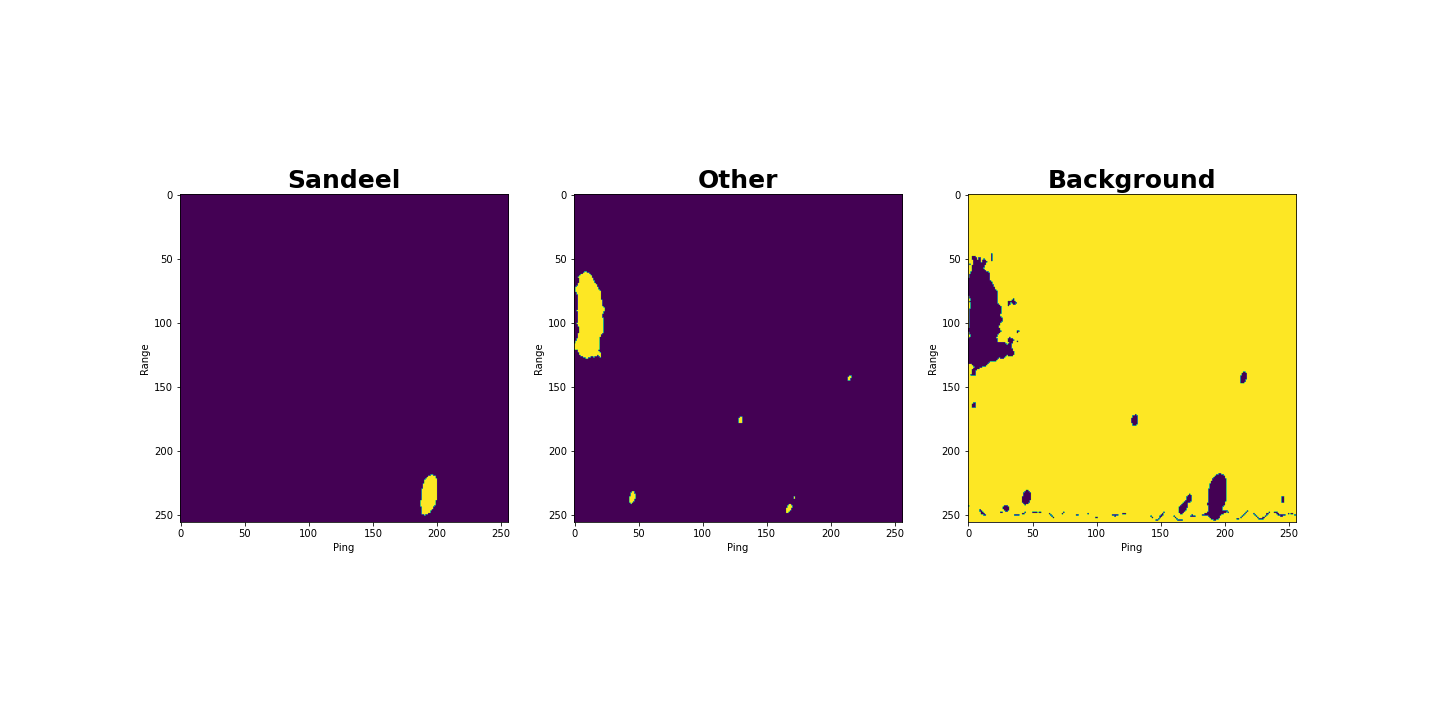
\includegraphics[width=1\textwidth]{figures/data_sample.png} } 
       % 
       % \subfloat[Color channels RGB that forms a picture.]{
       % 	\includesvg[inkscapelatex=false,width=0.9\textwidth,keepaspectratio]{figures/color%s_and_OG.svg}}
       % 
       % 
       % \caption[Frequency channels and color channels]{(a) and (b) both consist of several %channels that together represent some visual observation. \textbf{Credit:} Charles J. %Sharp, CC BY-SA 4.0 <https://creativecommons.org/licenses/by-sa/4.0>, via Wikimedia %Commons}
       % \label{accoustic data and color channels fig}
       % 
       % \end{figure}
    
    %More information about the acoustic data used in this thesis is contained in section %\ref{unet_paper_acoustic}. 
    
    
\section{Acoustic Classification of Sandeel} \label{acoustic classification sandeel}

Acoustic target classification is a major challenge in most acoustic surveys, and the sandeel is known to be difficult to interpret\cite{sizedependentfreqrespons2009johnsen}. It has been shown that large schools of sandeel likely have a connection to the seabed, resulting in severe underestimates of such schools by conventional echosounders\cite{johnsen2017collective}. The earlier mentioned Norwegian sandeel surveys use the \textit{200kHz} frequency to delineate schools, while the \textit{18kHz} and \textit{38kHz} are the most important frequencies for classification when measurements were taken at \textit{18kHz}, \textit{38kHz}, \textit{120kHz}, and \textit{200kHz}\cite{sizedependentfreqrespons2009johnsen}. Some earlier work have had trouble identifying sandeel using \gls{sv} at \textit{38kHz} and \textit{120kHz}\cite{hassel2004influence,mackinson2005using,mosteiro2004dual}, while some have had success using combinations of the four frequencies \textit{18kHz, 38kHz, 120kHz, and 200kHz} to specifically separate sandeel from herring, and mackerel\cite{mohammed2006acoustic}. This thesis goal is to find the subset of frequencies that capture most information about the sandeel, and will perform the analysis through the use of \textit{deep learning}, a field within \textit{machine learning}.

%The sandeels lack of swim bladder gives it a low \gls{ts}, and a swimming pattern that is usually not horizontal, which causes problems as the angle of the fish can change the backscattered signal\cite{Forland2014Broadbandwidth}.

%Greenstreet


\section{Machine Learning} \label{Machine Learning}
    Machine learning can be split into four parts; the \textit{algorithm}, \textit{empirical data}, a \textit{task} and a \textit{performance} measure\cite{Goodfellow-et-al-2016_ML}. A machine learning algorithm is designed to increase performance on a task, given data. During this process also called \textit{training}, the algorithm is said to be \textit{learning} by fitting a \textit{model} to the data. The two machine learning approaches used in this thesis are: supervised learning, unsupervised\cite{Goodfellow-et-al-2016_E}. 
    
    
    \subsection{Algorithm approaches} \label{Algorithm types}
        \subsection{Supervised learning}
            Supervised learning  algorithms are defined by the training data consisting of an input and a desired output\cite{Goodfellow-et-al-2016_E}. This means that the algorithm will have to learn a function, mapping from input to correct output. In classification problems, the output would be a class label, which could be classifying pictures of cats from other animals. While in regression problems, the output is a value within a numerical range. For example, predicting the height of a person.
            
        \subsection{Unsupervised Learning}
            Unlike supervised leaning, unsupervised learning algorithms only receive the input and learn properties contained in the data\cite{Goodfellow-et-al-2016_E}. A practical example is clustering, where the samples in a dataset are divided into clusters of similar properties. 
                
        %\subsection{Reinforcement Learning}
            %In reinforcement learning \cite{Goodfellow-et-al-2016_E}, the algorithm does not learn from a given dataset, but acts in an environment. In some cases, this is a feedback loop, giving either a positive or negative reward for performing certain actions. Examples can be seen in the AlphaZero software that beat professional chess players\cite{silver2017mastering}.
    
    \subsection{Data and Features}
    The quality of the input data to a machine learning algorithm will likely affect its performance\cite{najafabadi2015deep}. Hence, time allocated to increase quality of the data can exceed the time spent learning.  Data must be gathered, integrated, cleaned of errors, preprocessed, and features extracted before being used in learning. The process of extracting features is often referred to as \textit{feature engineering}. It constructs a representation of the data with the most important factors to solve the task. This is often domain specialized, and usually requires human involvement. In section \ref{neural networks}, \gls{ann} are introduced, which is one avenue within machine learning to automate the extraction of complicated features representations.


\section{Artificial Neural Networks} \label{neural networks}
    In this section, we introduce the basic components of an \gls{ann} and how these are combined to create a \textit{deep learning} network/ model. 

    \subsection{Perceptron} \label{perceptron}
        The \gls{ann}s fundamental building block is called an artificial \textit{neuron} or perceptron. It consists of a linear regression with the tunable parameters $w$ and $b$ inside a non-linear activation function, which will be explained later in \ref{activation function}. The perceptron is formulated in the following way\cite{razavi2021deep_exp_per}:
            \begin{equation} \label{eq_perceptron}
                y = \sigma(\sum_{i=1}^{D}w_ix_i + b)
            \end{equation}
            
        where D is the number dimension of the input space, $x$ is the input vector and $w$ is a set of weights that is of the same size as $x$, $b$ is the bias and {\textsigma} is the activation function. The single output value \textit{y} is a weighted sum of the input and weights plus the bias, also called the neurons' \textit{activation}. The perceptron is illustrated in figure \ref{Perceptron / MLP}.
    
    \subsection{Multi-Layered Perceptron} \label{MLP}
        The neurons presented in section \ref{perceptron} are organized together in layers to form an \gls{ann}, which in turn forms what is called a \gls{mlp} \cite{razavi2021deep_exp_per}. If all neurons in each layer are connected to every neuron in the next layer, then they form a type of \gls{ann} called \textit{fully connected} networks. A \gls{mlp} is depicted in figure \ref{Perceptron / MLP}.
        
            \begin{figure}[H]
                \centering
                
                \subfloat[Perceptron/neuron.]{
        	\includesvg[inkscapelatex=false,width=0.4\textwidth,keepaspectratio]{figures/neuron.svg} \label{perceptron fig}}
        	
        	       \subfloat[A \gls{mlp} with four inputs in the input-layer(arrows to the left), two hidden layers(\textbf{h}), and three outputs in the output-layer($\hat{\textbf{y}}$).]{
        	\includesvg[inkscapelatex=false,width=0.5\textwidth,keepaspectratio]{figures/mlp.svg}\label{mlp fig}}
                %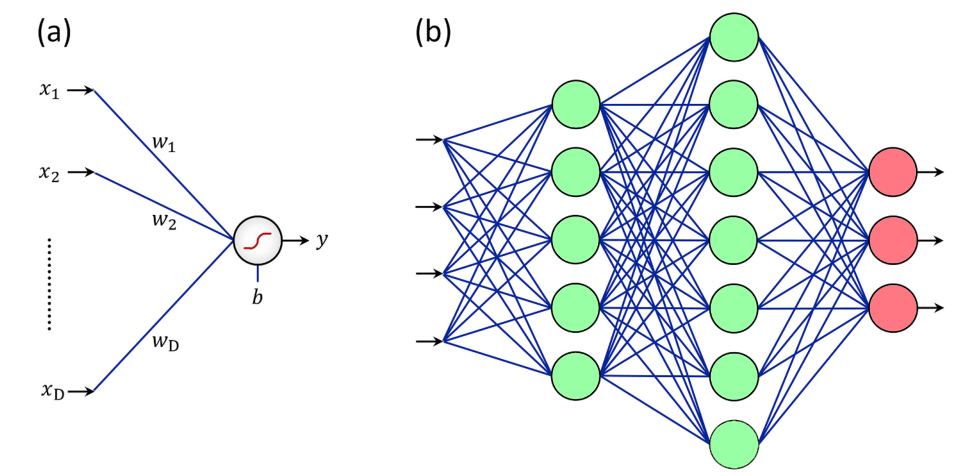
\includegraphics[scale=0.5]{figures/perceptron.png}
                
                \caption[The perceptron and multi-layer perceptron]{Illustration of a single neuron and a deep learning network of neurons.}
              	\medskip 
                \hspace*{15pt}\hbox{\scriptsize Credit: \citeauthor{razavi2021deep_exp_DL}\cite{razavi2021deep_exp_DL}}
                \label{Perceptron / MLP}
            \end{figure}
        
        The \textit{architecture} of any \gls{ann} consist of an input layer, a user-defined number of \textit{hidden layers} and finally an output layer\cite{razavi2021deep_exp_per}. More hidden layers form a \textit{deeper} network, hence the name \textbf{deep learning}. An \gls{mlp} is a type of network called a \textit{feed-forward} \gls{ann} because the data flows from the input to the output layer and each layer is a function of the previous layer. During training, the weights between every neuron and the bias are optimized in a process which is further explained in section \ref{training neural networks}. In the MLP depicted in \ref{Perceptron / MLP}, different neurons will activate with varying strengths depending on the input, resulting in different outputs. The architecture of the \gls{mlp} in figure \ref{Perceptron / MLP} can be expressed as\cite{Goodfellow-et-al-2016_architecture}:
        
        \begin{align}\label{mlp outputlayer eq}
            \textbf{h}^{(1)} &= \sigma^{(1)}(\textbf{W}^{(1)T}\textbf{x} + \textbf{b}^{(1)})\\
            \textbf{h}^{(2)} &= \sigma^{(2)}(\textbf{W}^{(2)T}\textbf{h}^{(1)} + \textbf{b}^{(2)})\\
            \hat{\textbf{y}} &= \sigma^{(3)}(\textbf{W}^{(3)T}\textbf{h}^{(2)} + \textbf{b}^{(3)})
        \end{align}

        
        
%        \begin{equation}
%            \textbf{h}^{(1)} = \sigma^{(1)}(\textbf{W}^{(1)T}\textbf{x} + \textbf{b}^{(1)})
%        \end{equation}
%        \begin{equation}
%            \textbf{h}^{(2)} = \sigma^{(2)}(\textbf{W}^{(2)T}\textbf{h}^{(1)} + %\textbf{b}^{(2)})
%        \end{equation}
%        \begin{equation} \label{mlp outputlayer eq}
%            \hat{\textbf{y}} = \sigma^{(3)}(\textbf{W}^{(3)T}\textbf{h}^{(2)} + %\textbf{b}^{(3)})
%        \end{equation}
        
        where for each layer \textbf{h} is a vector of activations, \textbf{W} is a vector of weights, \textbf{b} is a  vector of \textbf{biases}, and $\hat{\textbf{y}}$ is a vector of outputs. %The activation function $\sigma$ can also vary from layer to layer.
        
        
    \subsection{Activation Function} \label{activation function}
        The activation function enables \gls{ann}s to learn non-linear features \cite{razavi2021deep_exp_per}. The reason it is needed is that a network consisting of only linear layers will be the same as a single linear layer \cite{razavi2021deep_exp_per}. Hence, it won't be able to capture non-linearities in the data, and therefore an activation function is required in the hidden layers. Some activation functions can also be applied to the output of a network to solve the task the network is set to perform, and must be suited for the task at hand \cite{Goodfellow-et-al-2016_out_activation}. The activation function commonly used in the hidden layers is ReLU, which stands for \textit{rectified linear unit}\cite{sharma2019new_activation_func}. ReLU takes a real number as input, and outputs this number if it is above zero,  otherwise it will output zero. Letting $\sigma$ denote the activation function, and $x$ the input, the ReLU activation function can be formulated as follows:
            \begin{equation} \label{relu_eq}
                \sigma(x) = max(0,x)
            \end{equation}
        ReLU is also visualized in figure \ref{activation_fig}. This activation function allows some neurons to propagate their input, while preventing others from doing so. This can result in greater efficiency and faster training, as not all neurons are active, further detailed in \citeauthor{sharma2019new_activation_func}\cite{sharma2019new_activation_func}. 
        
        The logistic sigmoid activation function transforms all input values to values in the range [0…1].\cite{sharma2019new_activation_func}. It could be applied to the output to solve binary classification problems, as the values can be treated as probabilities. The formula for logistic sigmoid is:
            \begin{equation} \label{sigmoid_eq}
                \sigma(x) = \dfrac{1}{1 + e^{-x}} 
            \end{equation}
            
            \begin{figure}[H]
                \centering
                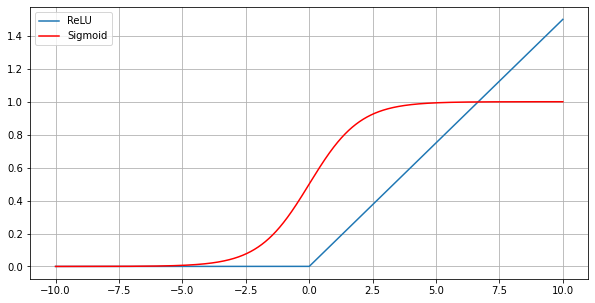
\includegraphics[scale=0.5]{figures/activation.png}
                \caption[ReLu and sigmoid]{A ReLU function (blue) and a sigmoid function (red)}.
              	\medskip 
                \label{activation_fig}
            \end{figure}

    \subsubsection{The Softmax Function}
        The \textit{softmax} can be viewed as a multivariate version of the logistic sigmoid activation function, which allows the softmax to be applied to problems containing multiple classes\cite{sharma2019new_activation_func}. For all data points, it calculates the probability of every class and can be expressed as:
        \begin{equation}
            \sigma(\textbf{x})_{j} = \dfrac{e^{x_{j}}}{\sum^{K}_{k=1}e^{x_{k}}} \textrm{ for j = 1,...,K.}
        \end{equation}
        
        where K is the number of classes and the output summarizes to 1 over all classes. For a network solving multiclass classification, the output layer will have size equal to K. This would corresponds to 3 classes in figure \ref{Perceptron / MLP}. The \textit{softmax} would then be used as the last transformation ($\sigma^{(3)}$ in equation \ref{mlp outputlayer eq}) and output the probability of an input belonging to one of the three classes.
        
\subsection{Convolutional Neural Network} \label{cnn}
    The \gls{cnn} is a type of \gls{ann} that is primarily used in machine learning tasks concerning images\cite{o2015introduction_convolutions}. One of the reasons for why the \gls{cnn} emerged was because images input to a regular \gls{ann} produces a large amount of learnable parameters. For example, a low-resolution image with $512\times512$ pixels passed to an input layer containing only one neuron would have $1\times512\times512 = 262144$ weights alone.  To solve this issue and have fewer learnable parameters, the modern \gls{cnn} is built around 3 main components\cite{o2015introduction_convolutions}; \textit{convolutional layer}, \textit{pooling layer} and a \textit{fully-connected layer}. An example \gls{cnn} is illustrated in figure \ref{convolutional_neural_network_fig} and each main component will be explained later in this section.

    \begin{figure}[H]
        \centering
                        \includesvg[inkscapelatex=false,width=0.95\textwidth,keepaspectratio]{figures/conv_net.svg}
        \caption[Convolutional neural network example]{Illustrations of the main components in a \gls{cnn}.}
      	\medskip 
        \label{convolutional_neural_network_fig}
    \end{figure}

%The \textit{flatten} operation is applied here to make the output from the pooling layer compatible with the fully connected layer of regular neurons.


    \subsubsection{Convolutional Layer}
    
    
     \citeauthor{o2015introduction_convolutions}\cite{o2015introduction_convolutions} describe the convolutional layer as consisting of a number of learnable multidimensional weight matrices which slides over the input. We will refer to such a matrix as a kernel. The height and the width of the kernel are parameters defined by the user, but the depth will always be equal the number of channels in the input. This results in kernels being described only by $height \times width$. The kernel slides over the input, and is applied to different locations of the input, also called the current \textit{receptive field}. When applied, a single scalar value is computed which is the weighted sum of the kernel's weights and the corresponding values in the receptive field. If we have a 2-dimensional image $I(i,j)$ as input, a convolutional operation would be expressed as\cite{Goodfellow-et-al-2016_convolution}:
     
        \begin{equation}
            (I*K)(i,j) = \sum_{height}\sum_{width}I(i+height,j+width)K(height,width)
        \end{equation}
     
     where $*$ is the convolutional operation, \textit{I(i,j)} is the image pixel at \textit{(i,j)}, and \textit{K} is the kernel.
     
     The output scalar value from the convolutional operation is often fed through non-linear activation functions like ReLU, and then called the \textit{activation}. The sliding operation is based around a value called \textit{stride}, which is the number of horizontal positions to move the kernel in the input between each calculation. If it is not possible to move in the horizontal direction, the kernel will move rows down vertically equal to the stride and then continue horizontally. After sliding over the entire input, a complete 2-dimensional activation map has been created, one such map for each kernel applied. The idea is that each of the applied kernels will learn to identify different features in the input. An example of a horizontal edge detector can be seen in figure \ref{convolutional_fig}\cite{o2015introduction_convolutions}. 
    \begin{figure}[H]
        \centering
                \includesvg[inkscapelatex=false,width=1\textwidth,keepaspectratio]{figures/convolutions.svg}
        \caption[Horizontal edge detector example]{Illustration of a \textit{valid} (detailed later in this section) convolutional operation. The kernel is applied repeatedly across the input. The size of input is 6×6, kernel size is 3×3 and stride 1, resulting in overlapping operations and output size being 4×4. The figures to the right show the input, kernel and output(activation) as color gradings, where the color gets darker if the values are low. This example is a horizontal edge detector, and the result is large values in the activation map along the border between the values of 0 and 10 in the input, which could have been colors in a picture.}
      	\medskip 
        \label{convolutional_fig}
    \end{figure}
    
    The receptive field will start as small regions, but as we apply more convolutional layers, it will have access to increasing context in regard to the input\cite{Goodfellow-et-al-2016}. This is illustrated in figure \ref{receptive_field_fig}, and kernels in early layers learn to identify simple features while later combine these to identify complex features. The kernel utilizes what is called \textit{parameter sharing }, as the same weights are repeatedly used across the input. The kernel is often smaller than the input, resulting in \textit{sparse connections} as opposed to fully connected networks. The parameter sharing results in the \gls{cnn} having another useful attribute called \textit{equivariance}, which means that if the input changes, the output changes in the same way.
    %which is that the location of the feature in the input is not relevant to a convolutional neural network. %Combined, this creates a layer able to detect features in an input with fewer learnable parameters than a normal \gls{ann}. 
    
    \begin{figure}[H]
        \centering
        \includesvg[inkscapelatex=false,width=0.9\textwidth,keepaspectratio]{figures/receptive_field_clown.svg}
        
        \caption[Receptive field]{The activation maps from two convolutional layers with 3×3 kernels and stride 1. The first convolution's receptive field is marked as red. On its activation map, a new convolutional layer is applied. Its first receptive field is outlined in green, which translates to a larger area in the input.}
      	\medskip 
        \hspace*{15pt}\hbox{\scriptsize Credit: Original image by Nick Hobgood\cite{clownfish_image}, used as input picture above (Edited with colored grid).}
        \label{receptive_field_fig}
    \end{figure}

    %The complete \textit{convolutional operation} performed by a convolutional layer consists of applying this kernel to the entire input. Producing activations for different regions of the input. This reduces the dimension of the input to a 2D activation output, but you may apply several kernels to increase the channels, as each will create a new 2D channel in the activations. A convolutional operation is often followed up with an element wise nonlinear activation function to its activations, like a ReLu. The kernels will through training learn to detect different features in the input, and so in a \gls{cnn} the first layers will often detect simple features like edges. Later layers will then detect more complex features like cars and houses, combining the activations from different earlier layers. The last layer consists of a \textit{fully connected} layer of regular neurons to determine the output, but implementations of networks with only convolutional operations exists like U-Net which will be described\cite{unet_ronneberger2015} in section \ref{unet} utilizing 1x1 convolutions. A more detailed example can be found in figure \ref{convolutional_fig} which looks at how a convolution with a horizontal edge detecting kernel is applied to a single channel or an equivalent 2D input. 
    
    Reductions in the spatial size will normally occur with the convolutional operation described so far in this section, such operations are called \textit{valid convolutions}\cite{o2015introduction_convolutions}. By applying a padding with zeros around the input, we can retain the dimensions of the input. The effect is that more convolutional operations fit in the new padded input, hence an equal output size. This is called a \textit{same convolution}. Illustrated in figure \ref{same_convolutional_fig}.
    
    \begin{figure}[H]
        \centering
        \includesvg[inkscapelatex=false,width=0.9\textwidth,keepaspectratio]{figures/same_convolutions.svg}
        \caption[Same convolution example]{Illustration of a \textit{same} convolutional operation. The size of the input is 3×3, but after padding with zeros the size is 5×5, kernel size is 3×3 and stride is 1. Resulting in an activation map if size 3×3, hence conserving the input size.}
      	\medskip 
        \label{same_convolutional_fig}
    \end{figure}
    
    
    
\subsubsection{The Max Pool Layer}

    \begin{figure}[H]
        \centering
                \includesvg[inkscapelatex=false,width=0.8\textwidth,keepaspectratio]{figures/maxpool.svg}
        \caption[The max pool operation]{Illustration of the max pool operation with size 2×2 and stride 2.}
      	\medskip 
        \label{maxpool_fig}
    \end{figure}
    The max pool layer reduces the \textit{height} and \textit{widht} of its input\cite{o2015introduction_convolutions}. Like a convolutional operation, the max pool looks at a region of the input, but instead applies a \textit{max} operation. The pooling kernel size is given in $height \times width$, and is applied individually to each dimension of the input. This reduces the height and width, but preserves the number of channels. The most common max pool layer is a 2×2 with a stride 2, which results in decreasing the resolution to 25\% of the original size. Alone, the max pool has no learnable parameters and is applied with the purpose of decreasing the computation complexity of the \gls{cnn}.


\subsubsection{Fully Connected Layer}
    \begin{figure}[H]
        \centering
        \includesvg[inkscapelatex=false,width=0.95\textwidth,keepaspectratio]{figures/1x1.svg}
        %\includesvg[inkscapelatex=false,scale=0.3,keepaspectratio]{figures/Bilde1.svg}
        \caption[1×1 convolution]{Illustration of the 1×1 convolution with stride 1.}
      	\medskip 
        \label{1x1_fig}
    \end{figure}
    \citeauthor{lin2013network_in_network_1x1}\cite{lin2013network_in_network_1x1} proposed the convolutional layer with kernel size 1×1 and stride 1, followed by an activation function. The 1×1 layer will take the weighted sum along a 1×1 slice through all channels of the input, as illustrated in figure \ref{1x1_fig}. This is equivalent to applying a fully connected layer to the same values. As this preserves the \textit{resolution}, it can be used as a tool for alterations of the depth of the output feature maps by specifying the desired number of kernels. In figure \ref{1x1_fig} we have only one kernel, but if two were applied instead, the output feature map would have a depth of two. In this work, it is used mainly to map high dimensional feature maps to the desired number of classes.
    
    
    %This is equivalent to the regular hidden layer shown earlier in figure \ref{Perceptron / MLP}, but for one pixel across the channels of the input.

\subsubsection{Transposed Convolutions}
    \begin{figure}[H]
        \centering
        \includesvg[inkscapelatex=false,width=0.95\textwidth,keepaspectratio]{figures/transpose_conv.svg}
        
        
        \caption[Transposed convolution]{Illustration of the transposed convolution operation with kernel size 2×2 and stride 1. The green color shows one of the intermediate computations. The center value of each crop is outlined to illustrate the summation step as these overlap.}
      	\medskip 
        \label{transposed_conv_fig}
    \end{figure}
    A transposed convolution is an operation taking an input, and with a kernel similar to that described in \ref{cnn}, but now instead map the input to a higher resolution\cite{dumoulin2016guide_transposed_convolution}. In example figure \ref{transposed_conv_fig}, a 2-dimensional 2×2 input is fed to a transposed convolutional layer with kernel size 2×2. The whole kernel is multiplied element-wise with the input and proceeds to produce values in a temporary matrix initialized with zeros, denoted by empty cells in the figure. In practice, we do not use the temporary values, but they are used here to illustrate the intermediate computations. The calculated values in the temporary matrix are situated correctly relative to the input. These temporary matrices are then summed over, producing the output. This operation is repeated for all channels, retaining the depth of the input. 
            


\subsubsection{Segmentation}
    \begin{figure}[H]
        \centering
        \includesvg[inkscapelatex=false,width=1\textwidth,keepaspectratio]{figures/segmentation_clown.svg}
        \caption[Difference between semantic and instance segmentation]{Illustration of the difference between semantic and instance segmentation.}
      	\medskip 
        \hspace*{15pt}\hbox{\scriptsize Credit: Original image (\textit{Input picture above}) by Nick Hobgood\cite{clownfish_image}}
        \label{segmentation_fig}
    \end{figure}

    Segmentation is a task where the objective is to assign one or several classification masks to the input\cite{He_2017_ICCV_segmentation}. This is further split into two different categories: \textit{semantic} and \textit{instance} segmentation. In semantic segmentation, we assign each pixel in the input to predefined classes. The output would have the same resolution as  the input, but with depth equal to the number of classes. A softmax would then be calculated for each pixel across the depth, and the pixel would be assigned to the class with the highest probability. Hence, producing a mask of each class. In instance segmentation, we increase the complexity by applying semantic segmentation while in parallel assigning a bounding box to each individual object, as visualized in figure \ref{segmentation_fig}.
    
\section{Training Neural Networks} \label{training neural networks}
    This section will describe the main concepts behind how neural networks are trained to perform on various tasks. 

\subsection{Forward-Propagation and The Loss Function}
    %    A \gls{ann} can be  described as an unknown function \textit{\^{f}} that maps an input \textbf{x} to an output \textbf{y}\cite{Goodfellow-et-al-2016_NN}. 

    The objective of an \gls{ann} is to approximate some optimal function \textit{f}, and in this thesis, we focus on classifiers, $\textbf{y} = f(\textbf{x})$ which maps an input \textbf{x} to an output category \textbf{y}. The \gls{ann} approximates this function by defining a mapping, $\textbf{\^{y}} = \hat{f}(\textbf{x},\theta)$ and learns the values of the parameters \textit{$\theta$} (weights and biases) through training using examples. In supervised tasks, the labels instruct the output layer exactly how to perform given the input data. However, the data does not inform the individual \textit{hidden layers} how to behave to produce this desired output. When the data flow through the network using the parameters $\theta$, it produces outputs \textbf{\^{y}}, this is called the \textit{forward-propagation step}. How the parameters are initialized can heavily affect the training process, and different strategies are further described in \citeauthor{Goodfellow-et-al-2016_param_init}\cite{Goodfellow-et-al-2016_param_init}. By using a \textit{loss function} to compare the true \textbf{y} values to the estimated values \textbf{\^{y}}, we get a measurement of the network's \textit{error}, also called \textit{loss}. The network uses this loss to then alter $\theta$ to best approximate \textit{f}, which will be explained later in section \ref{backpropagation}. In classification tasks, the network is trained to output the probability of each class given an input\cite{ho2019real_weighted_cross_entropy}. To train such a model, we can use a loss function called \textit{weighted cross entropy}. This function outputs a loss based on the probabilities, weights classification of certain classes differently, and is often used when dealing with data containing class imbalance as you can apply more weight to the minority class. Expressed as:
    
        \begin{equation} \label{cross_entropy}
            loss(\theta) = - \sum^{n}_{i=1} w_{y_{i}}y_{i}\log(\hat{y_{i}})
        \end{equation}
    
    where \textit{n} is the number of classes, $y_{i}$ is 1 if the $i^{th}$ class is true (\textit{else 0}), $\hat{y_{i}}$ is the output from the softmax for the $i^{th}$ class, and $w_{y_{i}}$ is the weight of the class to which $y_{i}$ belongs. More examples of loss functions can be viewed in \citeauthor{mishra2017deep}\cite{mishra2017deep}.
    


\subsection{Mini-batch Stochastic Gradient Decent} \label{batch learning}
        \begin{quote}
        "\textit{A recurring problem in machine learning is that large training sets are necessary for good generalization, but large training sets are also more computationally
        expensive."} - (\citeauthor{Goodfellow-et-al-2016_SGD}\citeyear{Goodfellow-et-al-2016_SGD}, page 152)
    \end{quote}
    
    Calculating the total loss of the whole dataset is often unfeasible, and depending on the hardware, this could lead to a crash or slow learning due to
    heavy memory demands. A solution is to sample a set of examples, called a \textit{mini-batch}, from the entire dataset, with the intent to approximately estimate
    the true loss using this smaller fraction of the dataset. Then we update the parameters of our network based on this and repeat on a new batch. This is called mini-batch \textit{\gls{sgd}}, which is a common \textit{optimization} algorithm\cite{Goodfellow-et-al-2016_SGD}. The size of this mini-batch can vary from one example (\textit{also called true \gls{sgd}}), to hundreds, and the size chosen can heavily affect training\cite{wilson2001need_learning_rate}
    
    
    
    
    %The problem, described in the quote above, arises when we have a large dataset, and we would calculate the loss values of all samples before updating the parameters in our network\cite{Goodfellow-et-al-2016_SGD}. Depending on the hardware, this could lead to a crash or slow learning due to heavy memory demands. A solution is then to sample examples from the entire dataset with a uniform distribution, hence forming a \textit{mini-batch}, with the intent to approximately estimate the true \textit{loss} using this smaller fraction of the dataset. We can then update the parameters of our network based on this and repeat on a new batch. When we have run this process on all the data, we say that an \textit{epoch} has passed. . This algorithm is called \textit{\gls{sgd}}\cite{Goodfellow-et-al-2016_SGD}, which utilizes this minibatch form of training, and is used in this thesis. \gls{sgd} optimizes the parameters of the network by minimizing the loss\cite{pmlr-v37-ioffe15_batch_norm}:
    
        %\begin{equation} \label{batch_learning_eq}
            %\theta = \arg \min_{\theta}\dfrac{1}{N} \sum^{N}_{i=1} loss (x_{i},\theta)
        %\end{equation}
    
    %where $\theta$ is the set of parameters to be optimized, $x_{1..N}$ is the training data, and $x_{1..m}$ is a minibatch of the training data. \gls{sgd} is what is called an \textit{optimization} algorithm.
    
    
\subsection{Backpropagation and Gradient-based Learning}\label{backpropagation}
    To update the parameters of the network, we use the loss from a mini-batch, and iteratively step back through the layers in a process called \textit{back-propagation}\cite{rumelhart1986learning_backprop}. In each step, we calculate a value called the \textit{gradient} for each parameter. The gradient is the partial derivative of the \textit{loss} function with respect to each weight and bias in the current layer, and is computed using the chain rule. This is in order to determine how changes to each parameter will affect the \textit{loss}. Using the gradient, \gls{sgd} performs \textit{gradient descent}\cite{Goodfellow-et-al-2016_gradient_descent} by updating all parameters in the opposite direction of the gradient to reduce the loss. In what magnitude a parameter is adjusted by the optimizing algorithm is determined by the \textit{learning rate}, usually a value between 0 and 1. The parameter update is expressed as\cite{pmlr-v37-ioffe15_batch_norm}:
    
    \begin{equation}
    \theta^{(j)} \leftarrow \theta^{(j)} - \eta \dfrac{1}{m}\sum_{i=1}^{m} \dfrac{\partial loss (\theta^{(j)})}{\partial \theta^{(j)}}
    \end{equation}
    
    where $\theta$ is the parameters of the network, \textit{m} is the batch size, $\eta$ is the learning rate, and \textit{j} is the layer. In figure \ref{learning_rates} an example loss function is illustrated with one global \textit{loss} minima, and different learning rates applied with \gls{sgd}. Low learning rate values usually have a long training time, and may cause the \gls{sgd} to converge to a local minima instead of the global\cite{farsal2018deep}. However, too high values can overshoot the global minima and diverge. Both can be prevented by applying a method to adapt the learning rate to the \textit{topography} of the loss function. In this thesis, \textit{momentum} was applied, which only acts as a \textit{velocity} to the update step. This \textit{velocity} is based on past steps and the update will step in the \textit{velocities'} direction, not the current \textit{gradient}. More detail on \textit{momentum} can be found in \citeauthor{pmlr-v28-sutskever13}\cite{pmlr-v28-sutskever13}.
    
    \begin{figure}[H]
        \centering

        \includesvg[inkscapelatex=false,width=1.0\textwidth,keepaspectratio]{figures/learning_rates.svg}
        \caption[Learning rates]{Three different applications of \gls{sgd} on a loss function . Each arrow is an imagined learning step taken by the algorithm for; (a) low learning rate, (b) high learning rate, and (c) momentum.}
      	\medskip 
        \label{learning_rates}
    \end{figure}

    In summary, the entire training process using \gls{sgd} can be described as the following algorithm\cite{farsal2018deep}:
    
    \begin{longtable}{lllllll} \label{sgd algorithm}\\
    \hline
    \multicolumn{7}{l}{Mini-batch SGD one epoch}                                                              \\ \hline
    \endfirsthead
    %
    \endhead
    %
    \hline
    \endfoot
    %
    \endlastfoot
    %
    \multicolumn{7}{l}{Loop:}                                                                       \\
    1.   & \multicolumn{6}{l}{Sample batch of data.}                                                \\
    2.   & \multicolumn{6}{l}{Forward propagate the batch through the network and compute the loss.} \\
    3.   & \multicolumn{6}{l}{Back propagate to calculate the gradients.}                            \\
    4.   & \multicolumn{6}{l}{Update the parameters based on the gradients.}                         \\ \hline
    \end{longtable}
    
    

%\subsection{Vanishing and exploding gradient} \label{}
    %By repeatedly applying forward-propagation, back-propagation and some optimizing algorithm on new examples as stated by \citeauthor{Goodfellow-et-al-2016_NN}, you train a network to approximate the optimal function \textit{f}.
\section{Model Evaluation}
    To evaluate a machine learning algorithm, we need a performance measure. First, the \textit{performance metric} itself will be described, followed by a technique applied to make unbiased measures of the model by leaving our parts of the data. Finally, two central challenges that appear in machine learning.
    
    \subsection{Performance Metrics} \label{f1_score}
        This section describes the performance metrics used in this thesis. Consider a binary classification system that classifies samples into either the \textit{positive} or \textit{negative} class. Predictions by the classifier can thus be sorted into the following four categories\cite{powers2020evaluation_f1_recall_precision}:
        
        \begin{itemize}
            \item \textbf{True positive (TP):} A correct classification of a positive example.
            \item \textbf{True negative (TN):} A correct classification of a negative example.
            \item \textbf{False positive (FP):} A negative example incorrectly classified as positive
            \item \textbf{False negative (FN):} A positive example incorrectly classified as negative.
            \end{itemize}
        
        We can now calculate the performance of the classifier from these values, and the simplest is accuracy\cite{powers2020evaluation_f1_recall_precision}:
        
        \begin{equation}
            accuracy = \dfrac{\textrm{\textit{correct predictions}}}{\textrm{\textit{total number of predictions}}} = \dfrac{TP+TN}{TP+TN+FP+FN} 
        \end{equation}
        
        This metrics does not handle class imbalance well, as it is equivalent to calculating the percentage of correct predictions\cite{powers2020evaluation_f1_recall_precision}. An example being that if 95\% of the data belongs to one class, then always predicting this class will give us an accuracy of 95\%.
        
        To deal with class imbalance, we calculate two new metrics, \textit{precision} and \textit{recall}\cite{powers2020evaluation_f1_recall_precision}. Precision is the percentage of positive predictions made by the model that are correct. Recall is the percentage of all positive samples the model managed to classify correctly.
        
        \begin{equation}
            \textrm{\textit{precision}} = \dfrac{TP}{TP+FP}
        \end{equation}
        
        \begin{equation}
            \textrm{\textit{recall}} = \dfrac{TP}{TP+FN}
        \end{equation}
        
        Then, by using precision and recall, we calculate the \textit{F1-score}\cite{powers2020evaluation_f1_recall_precision}. It combines these metrics and is designed to work well on imbalanced data. The F1-score formula: %There are of course many other performance metrics, but this section will be limited to describing those used in the thesis. 
        
        \begin{equation}
            \textrm{\textit{F1-score}} = 2 \cdot \dfrac{\textrm{\textit{precision}} \cdot \textrm{\textit{recall}}}{\textrm{\textit{precision}} + \textrm{\textit{recall}}}
        \end{equation}
        
    \subsection{Train-Validation-Test Split}
        The goal when a machine learning model is learning, is to achieve the lowest \textit{generalization error}\cite{Goodfellow-et-al-2016_generalization}. This means to not only perform well on data seen during training, but also on new unseen data. To measure this error, it is normal to split our data into three parts\cite{Goodfellow-et-al-2016_train_val_test_split}: the \textit{training}, \textit{validation} and \textit{test} dataset, and we measure some error on each. As the name suggests, the training data is used during the training process of the model. The validation dataset, is extracted from the training dataset and gives an unbiased estimate of the models' performance and can be used to guide the training process. The last mentioned could be to select the best model from a selection of many. Finally, the test dataset is used to get an unbiased estimate of the final model's \textit{generalization error}.
        
    
    \subsection{Overfitting Vs. Underfitting}
        The performance of a model is dependent on its \textit{training error}, and the difference between this \textit{training error} and the \textit{test error}. \textit{Underfitting} happens when a model fails to achieve a low training error, while \textit{overfitting} happens when the difference between the test error is significantly lower than the training error. To manipulate this behavior, we adjust the models \textit{capacity}. Capacity represents the variety of functions the model is able to learn, and by adjusting it one can increase and decrease the likelihood of underfitting and overfitting. The capacity can be controlled by, for example, changing the number of layers in a neural network, and further details can be seen in \citeauthor{Goodfellow-et-al-2016}\cite{Goodfellow-et-al-2016}. Low \textit{capacity} means that the model may fail to capture patterns contained in the data. High \textit{capacity} translates to adjusting to the training data to such an extent that the model performs may be worse when given unseen test data. The optimal solution, depicted in the center plot of figure \ref{over/under fit fig}, is to have a model with a balanced capacity that is as close to the true function as possible\cite{Goodfellow-et-al-2016}. 
        
       % \citeauthor{Goodfellow-et-al-2016}\cite{Goodfellow-et-al-2016}
        
        \begin{figure}[H]
            \centering
            %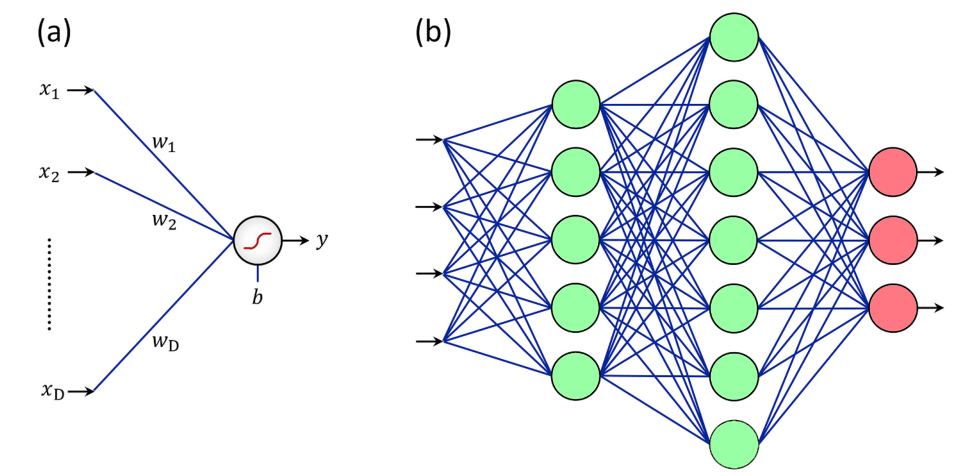
\includegraphics[scale=0.5]{figures/perceptron.png}
            \includesvg[inkscapelatex=false,width=1\textwidth,keepaspectratio]{figures/overunderfit.svg}
            \caption[Over/under-fit]{Training data is generated with random noise around a sinus wave (True function). Model \textit{capacity} increases from left to right. The center plot illustrates a model that have learned an almost perfect fit to the actual true function.}
          	\medskip 
            \label{over/under fit fig}
        \end{figure}
        
        
\todo{skrive om hyperparameter?}
\section{Regularization}
    Regularization as described by \citeauthor{kukavcka2017_regularization}\cite{kukavcka2017_regularization} is any supplemental technique with the goal to increase the model generalization performance. Two techniques used in this thesis will be described here; \textit{batch normalization} and \textit{data-augmentation}.
    
\subsection{Batch-Norm}
    Batch normalization is a technique applied to reduce what is called \textit{internal  covariate shift}\cite{pmlr-v37-ioffe15_batch_norm}. This is defined as the change in the distribution of activations in hidden layers caused by the change in the networks parameters when training. During \textit{backpropagation}, the hidden layers depend on the activations of all layers before them, and as each of them change their output distribution, the other layers have to adapt to this change. Research has shown that this slows down and destabilize the training process, and a solution to this problem is the implementation of \textit{batch normalization}. By using the activations from all the neurons in a hidden layer, a \textit{mean} and \textit{variance} is calculated per batch. These values are then used to normalize the activations of the hidden layer. Each hidden layer are given two additional learnable parameters $\gamma$ and $\beta$, that perform a linear transformation of the normalized activations, defined as such:
    
        \begin{equation} \label{batch_normalization}
            \hat{Z}^{(i)} =   \gamma Z^{(i)}_{norm} + \beta
        \end{equation}
    
    where $\hat{Z}^{(i)}$ is the batch normalized activations, $Z^{(i)}_{norm}$ is the normalized activations for the $i^{th}$ hidden layer. The learnable parameters make the \gls{ann} able to adjust and shift the distribution through the training process. The result may lead to a faster and more stable training process. 
    
    Recently, the poor understanding of batch normalization has come into question and \citet{batch_norm_not_work} has stressed that more investigation should be put into understanding its effectiveness. Their findings showing that it might not stem from internal covariate shift, but other factors. 

\subsection{Data-Augmentation} \label{data-augmentation}
     \textit{Data-augmentation} is a regularization method that is directly applied to the training dataset\cite{kukavcka2017_regularization}. This is done by applying some transformation to the training set. There are several methods available, but the two used in this work are: \textit{adding noise} and \textit{vertical flipping}. One example of applying noise is to add Gaussian values with a mean of 0 and some user-defined variance to each pixel. This adds more randomness to the data, making the model learn more general features instead of specific. The network is less prone to overfit on certain samples, which in turn might increase generalization performance. Other methods of applying noise are described in \citeauthor{kukavcka2017_regularization}\cite{kukavcka2017_regularization}. Vertical flipping is a simple transformation where we flip the input and label along a certain axis. Thus, mapping the data to a new representation. An example of each method mentioned can be seen in figure \ref{data augmentation fig}:
    % This is an important observation when applying data augmentation, as it can't change the meaning of the data. For example, when classifying numbers in images, rotating an image of the number \textit{9} clockwise 180 degrees will change its representation to now be more similar to a \textit{6}, but the label would still claim it belongs to the class \textit{9}.
    \begin{figure}[H]
        \centering
        
        \subfloat[Gaussian noise added to each pixel.]{
        	\includesvg[inkscapelatex=false,width=0.9\textwidth,keepaspectratio]{figures/add_noise_clown.svg}}
        	%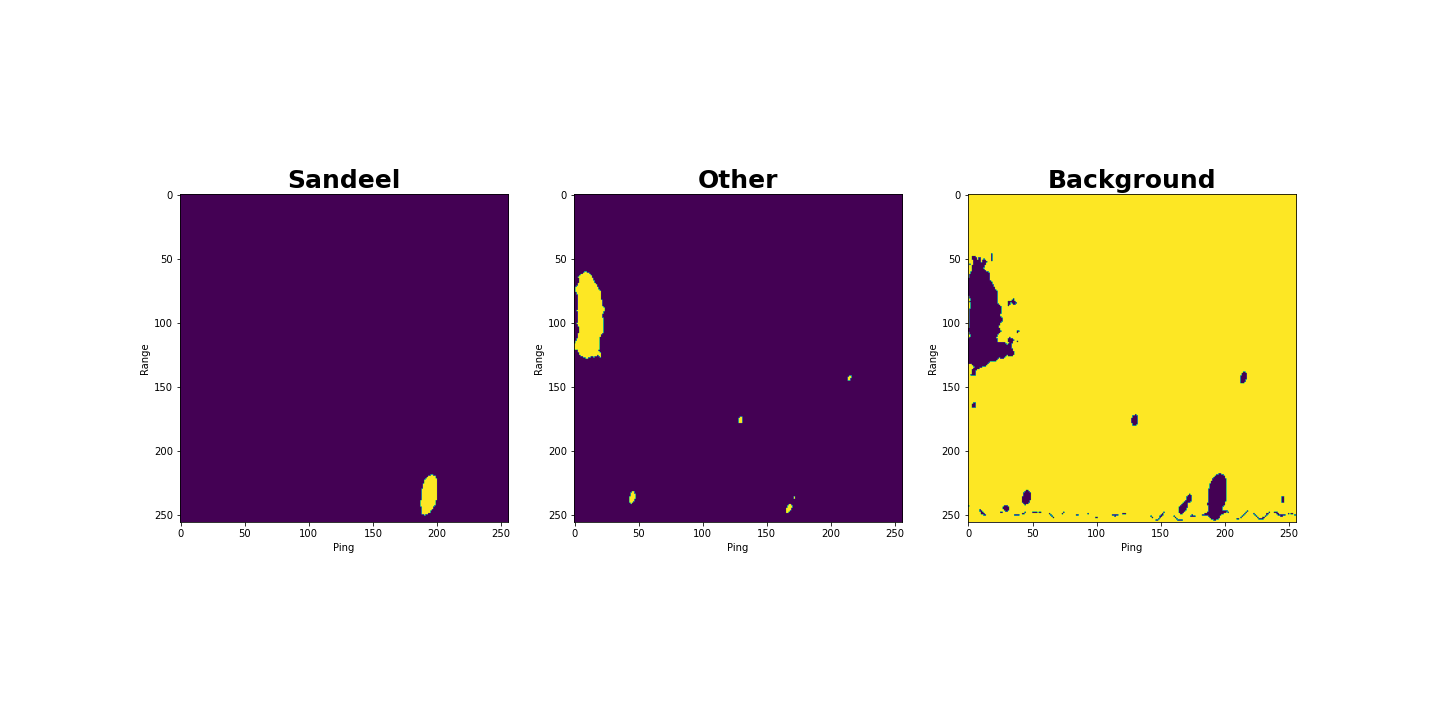
\includegraphics[width=1\textwidth]{figures/data_sample.png} } 
        
        \subfloat[Vertical flipping.]{
        	\includesvg[inkscapelatex=false,width=0.9\textwidth,keepaspectratio]{figures/vertical_flip_clown.svg}}
        
        
        \caption[Two data augmentation examples]{Two augmentation methods applied to the same image.}
        \medskip 
        \hspace*{15pt}\hbox{\scriptsize Credit: Original image (\textit{Both left pictures above}) by Nick Hobgood\cite{clownfish_image}}
        \label{data augmentation fig}
        
        \end{figure}
    

\section{U-Net} \label{unet}

    In this section, we introduce the architecture of the model that is the backbone of the work in this thesis. U-Net is a fully convolutional, state-of-the-art\cite{rajak2021segmentation} semantic segmentation \gls{cnn} initially developed for biomedical image analysis by \citeauthor{unet_ronneberger2015}\cite{unet_ronneberger2015}. 
    
    \begin{figure}[H]
        \centering
        %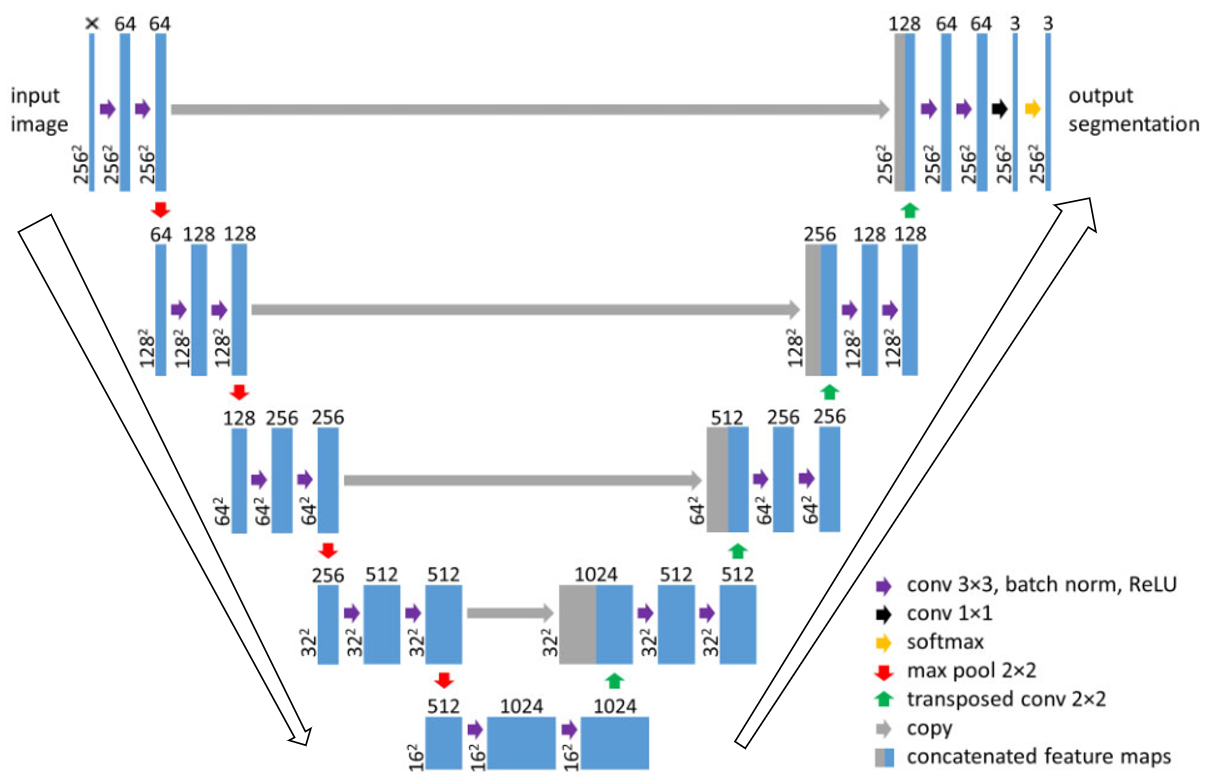
\includegraphics[scale=0.5]{figures/unet_arrows.png}
        \includesvg[inkscapelatex=false,width=1.0\textwidth,keepaspectratio]{figures/unet_original.svg}
        \caption[U-Net architecture]{U-Net architecture, the downwards facing arrow illustrates the contracting path and the one facing upwards is the expanding path. The color gets darker as the channels increase.}
      	\medskip 
        \label{unet_fig}
        \hspace*{15pt}\hbox{\scriptsize Credit: \citeauthor{unet_ronneberger2015}\cite{unet_ronneberger2015}}
    \end{figure}
    
    %Each stage applied the same operations to its given input.
    
    U-Net utilized what \citeauthor{unet_ronneberger2015}\cite{unet_ronneberger2015} called a \textit{contracting path} to identify what was in a picture, while an \textit{expanding path} localized where it was. These two branches were symmetrical, and together they formed a U-shape, giving the network its name. The contracting path can be looked at as five different stages of processing, from top to bottom, in figure \ref{unet_fig}. For each stage, this consisted of two 3×3 valid convolutions with their individual ReLU activation functions. Initially, the feature channels would be increased to 64, then the channel would be further doubled for each contracting stage. The convolutions were followed by a 2×2 max pooling operation with stride 2 to further decrease the resolution of the output from the convolutional operations, and then output a feature map to the next stage. After the bottom stage, the max pool operation is replaced with transpose convolutions to now increase the resolution. At each subsequent stage traveling back up the expanding path, the number of feature channels is halved by the convolutional steps down to 64. 
    
    The output of the previous stage would be concatenated with a crop from the output feature map of a stage from the contracting path with the same channel size, the cropping is due to different resolutions. This step allows the following convolutional operation to access both the high-resolution feature map from the contracting path, and the upsampled feature map, which in combination helps with localization of features. 

    At the final layer in the expanding path, a 1×1 convolution maps the 64 feature channels to the 2 classes. Finally, the softmax was then calculated between these classes, giving each pixel a probability distribution over the classes, with one channel for each class. Hence, giving us a segmentation map.
    
    %Hence, these layers increase the resolution of the output. In order to localize, high resolution features from the contracting path are combined with the upsampled output. A successive convolution layer can then learn to assemble a more precise output based on this information.
    
    
    When released, U-Net outperformed other networks in multiple biomedical challenges\cite{unet_ronneberger2015}. It's performance inspired new models that use the U-Net architecture as their backbone, as can be seen in NAS-Unet\cite{weng2019unet} from \citeyear{weng2019unet}, and Unet++\cite{zhou2018unet} from \citeyear{zhou2018unet}. U-Net has also been applied with success to other fields such as road extraction in satellite images by \citeauthor{zhang2018road}\cite{zhang2018road} in \citeyear{zhang2018road} and on acoustic classification by \citeauthor{brautaset2020acoustic}\cite{brautaset2020acoustic} in \citeyear{brautaset2020acoustic}, which will be explained in the following chapter.
    
    %In the field of biomedicine, data are scarce and so heavy use of data augmentation was applied, which made the U-Net able to train on very few samples.
    
    %At the last stage, a 1×1 convolution was applied instead of increasing the resolution.





